\section{Hawker Siddeley Nimrod}

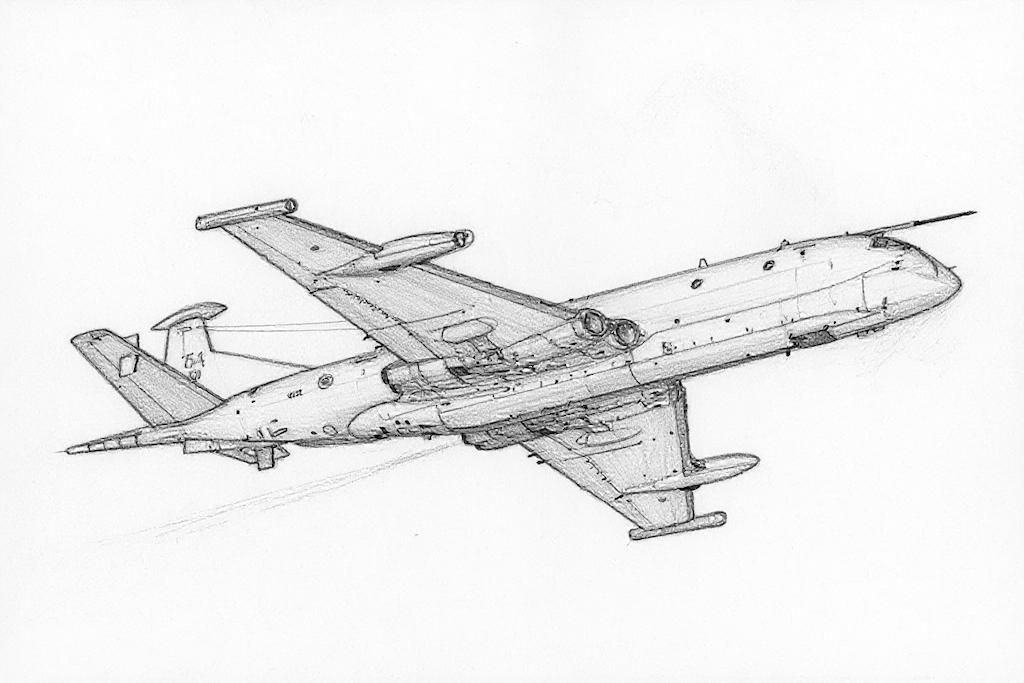
\includegraphics[width=\linewidth]{Nimrod.png}

The Hawker Siddeley Nimrod is a maritime patrol aircraft. It was developed from the Comet jet airliner, and this line thus holds the distinction of being both the first jet airliner and the first jet maritime patrol aircraft.

\subsection{Versions}

The initial Nimrod MR.1 reused many mission components from the Shackleton MR.3, in particular the ASV Mk~21 radar, and entered service with the RAF in 1969.

Many of the MR.1 aircraft were upgraded to the MR.2 standard starting in 1975, gaining the much improved Searchwater radar and Yellow Gate ESM system, and the remainder were retired.

During the South Atlantic War, air-to-air refueling probes from Avro Vulcans were installed on several MR.2s to give the MR.2P version and the underwing stations were equipped with AIM-9G/L IRMs. In 1990, some Nimrods were further equipped with decoy dispensers. In 2022, some gained TV/IR optics.

\subsection{ADCs}

ADCs are provided for:
\begin{adclist}
    \adcitem{Nimrod MR.1}
    \adcitem{Nimrod MR.2}
    \adcitem{Nimrod MR.2P}
\end{adclist}

\subsection{Photo Credit}
\begin{itemize}\raggedright
    \item \href{https://commons.wikimedia.org/wiki/File:British_Aerospace_Nimrod_MR.2,_United_Kingdom_-_Royal_Air_Force_(RAF)_JP506967.jpg}{Hawker Siddeley Nimrod}: Dale Coleman (GFDL 1.2)
\end{itemize}
